% !TeX encoding = UTF-8

%% ------------------------------------------------------------------------
%% Copyright (C) 2021-2023 SJTUG
%% 
%% SJTUBeamer Example Document by SJTUG
%% 
%% SJTUBeamer Example Document is licensed under a
%% Creative Commons Attribution-NonCommercial-ShareAlike 4.0 International License.
%% 
%% You should have received a copy of the license along with this
%% work. If not, see <http://creativecommons.org/licenses/by-nc-sa/4.0/>.
%%
%% For a quick start, check out src/doc/sjtubeamerquickstart.tex
%% Join discussions: https://github.com/sjtug/SJTUBeamer/discussions
%% -----------------------------------------------------------------------

\documentclass[xcolor=table,dvipsnames,svgnames,aspectratio=169]{ctexbeamer}
% 可以通过 fontset=macnew / fontset=ubuntu / fontset=windows 选项切换字体集;
% 如遇无法显示的数学符号,尝试对 ctexbeamer 文档类添加 no-math 选项;
% 写纯英文幻灯片可以改用 beamer 文档类。

\usepackage{tikz}
\usepackage[normalem]{ulem}
\usetikzlibrary{arrows}
\usepackage{amsmath}
\usepackage{graphicx}
\usepackage{hologo}
\usepackage{colortbl}
\usepackage{shapepar}
\usepackage{hyperxmp}
\usepackage{booktabs}
\usepackage{listings}
\usepackage{tipa}
\usepackage{multicol}
\usepackage{datetime2}
\usepackage{fontawesome5}
\usepackage{hyperref}

% 参考文献设置,使用 style=gb7714-2015 样式为标准顺序编码制,
% 使用 style=gb7714-2015ay 样式可以改为著者-出版年制。
% \usepackage[backend=biber,style=gb7714-2015]{biblatex}
% \addbibresource{ref.bib}

% 该行指定了图像的额外搜索路径
\graphicspath{{figures/}}

\hypersetup{
  pdfcopyright       = {Licensed under CC-BY-SA 4.0. Some rights reserved.},
  pdflicenseurl      = {http://creativecommons.org/licenses/by-sa/4.0/},
  unicode            = true,
  psdextra           = true,
  pdfdisplaydoctitle = true
}

\pdfstringdefDisableCommands{
  \let\\\relax
  \let\quad\relax
  \let\hspace\@gobble
}

% \renewcommand{\TeX}{\hologo{TeX}}
% \renewcommand{\LaTeX}{\hologo{LaTeX}}
% \newcommand{\BibTeX}{\hologo{BibTeX}}
% \newcommand{\XeTeX}{\hologo{XeTeX}}
% \newcommand{\pdfTeX}{\hologo{pdfTeX}}
% \newcommand{\LuaTeX}{\hologo{LuaTeX}}
% \newcommand{\MiKTeX}{\hologo{MiKTeX}}
% \newcommand{\MacTeX}{Mac\hologo{TeX}}
% \newcommand{\beamer}{\textsc{beamer}}
% \newcommand{\XeLaTeX}{\hologo{Xe}\kern-.13em\LaTeX{}}
% \newcommand{\pdfLaTeX}{pdf\LaTeX{}}
% \newcommand{\LuaLaTeX}{Lua\LaTeX{}}
% \def\TeXLive{\TeX{} Live}
% \let\TL=\TeXLive

% \newcommand{\SJTUThesis}{\textsc{SJTUThesis}}
% \newcommand{\SJTUThesisVersion}{2.0.3}
% \newcommand{\SJTUThesisDate}{2023/9/25}
% \newcommand{\SJTUBeamer}{\textsc{SJTUBeamer}}
% \newcommand{\SJTUBeamerVersion}{3.0.0}
% \newcommand{\SJTUBeamerDate}{2022/11/22}

% \newcommand\link[1]{\href{#1}{\faLink}}
% \newcommand\pkg[1]{\texttt{#1}}

% \def\cmd#1{\texttt{\color{structure}\footnotesize $\backslash$#1}}
% \def\env#1{\texttt{\color{structure}\footnotesize #1}}
% \def\cmdxmp#1#2#3{\small{\texttt{\color{structure}$\backslash$#1}\{#2\}
% \hspace{1em}\\ $\Rightarrow$\hspace{1em} {#3}\par\vskip1em}}

\usetheme[maxplus,blue,light]{sjtubeamer}
% \setbeameroption{show notes on second screen}
% 使用 maxplus/max/min 切换标题页样式
% 使用 red/blue 切换主色调
% 使用 light/dark 切换亮/暗色模式
% 使用外样式关键词以获得不同的边栏样式
%   miniframes infolines  sidebar
%   default    smoothbars split	 
%   shadow     tree       smoothtree
% 使用 topright/bottomright 切换徽标位置
% 使用逗号分隔列表以同时使用多种选项

% \setbeamertemplate{background}{}
% 对于 max 主题,如果需要关闭正文背景图,请取消注释上一行。

% \tikzexternalize[prefix=build/]
% 如果您需要缓存 tikz 图像,请取消注释上一行,并在编译选项中添加 -shell-escape。

\lstset{
  language=[LaTeX]TeX,           % 更改高亮语言
  texcsstyle=*\color{cprimary},  % 只在高亮 LaTeX 语言时必须
  tabsize=2,
  basicstyle=\ttfamily\small,%
  keywordstyle=\color{cprimary},%
  stringstyle=\color{csecondary},%
  commentstyle=\color{ctertiary!50!gray},%
  breaklines,%
}
\logo{}
\author{熊家辉}
\institute[萨塞克斯人工智能学院]{浙江工商大学}
% \date{\the\year 年 \the\month 月}
\date{2024 年 2 月 21 日}
% \date{\today}
\subject{Chisel 初体验}
\keywords{Chisel}

\title[Chisel 初体验] % 页脚显示标题
{\textbf{Chisel 初步探索与实验}} % 首页标题

\subtitle{PLCT Lab 每周技术分享}

\begin{document}

% 使用节目录
\AtBeginSection[]{
  \begin{frame}
    %% 使用传统节目录,也可以将 subsectionstyle=... 换成 hideallsubsections 以隐藏所有小节信息
    % \tableofcontents[currentsection,subsectionstyle=show/show/hide]
    %% 或者使用节页
    \sectionpage
  \end{frame}
}

% 使用小节目录
\AtBeginSubsection[]{		       % 在每小节开始
  \begin{frame}
    %% 使用传统小节目录
    % \tableofcontents[currentsection,subsectionstyle=show/shaded/hide]
    %% 或者使用小节页
    \subsectionpage
  \end{frame}
}

\maketitle

% \begin{frame}
%   \frametitle{来源}
%   \begin{thebibliography}{00}
%     \setbeamertemplate{bibliography item}[online]
%     \bibitem{} Alexara Wu.
%     \newblock 如何使用 \LaTeX{} 排版论文[EB/OL].
%     \newblock 2021.
%     \url{https://github.com/sjtug/sjtulib-latex-talk/tree/alexara-2021}
%   \end{thebibliography}

%   \vspace*{2ex}

%   \begin{itemize}
%     \item 本示例文档的源码结构适用于简短的单次报告,仅展示 \beamer{} 文档类的通
%           用功能,更多地在使用 \SJTUBeamer{} 的样式信息。
%     \item 为发挥 \SJTUBeamer{} 的全部功能,参见发布区
%           \link{https://github.com/sjtug/SJTUBeamer/releases} 的快速入门、用户手
%           册与开发文档。
%     \item 就制作一组讲座而言,相关源码结构可以参考新讲座
%           \link{https://github.com/sjtug/sjtulib-latex-talk/tree/logcreative-2022}。
%           新讲座使用了社区版主题的同时也展示了 \SJTUBeamer{} 的特殊用法。
%   \end{itemize}

% \end{frame}

\begin{frame}{目录}
  \tableofcontents[hideallsubsections]	% 隐藏所有小节信息
\end{frame}

\section{Verilog 语言简介}

\subsection{Verilog 语言}

\begin{frame}
  \frametitle{Verilog 语言}
  \begin{itemize}
    \item \paragraph{用途} Verilog 是一种用于描述、设计电子系统(特别是数字电路)的硬件描述语言,主要用于在集成电路设计,特别是超大规模集成电路的计算机辅助设计。
    \item \paragraph{标准} Verilog 是电气电子工程师学会(IEEE)的 1800-2009 号标准。
    \item \paragraph{语言要素} Verilog 的设计初衷是成为一种基本语法与 C 语言相近的硬件描述语言。
  \end{itemize}
\end{frame}

\begin{frame}[fragile]
  \frametitle{Verilog 代码示例}
  \begin{codeblock}[language=verilog]{一段由 Chisel 吐出的 Verilog 代码}
module ModuleSample(
  input        clock,reset,
  input  [7:0] io_a,io_b,
  output [7:0] io_minnum,io_maxnum
);
  wire _io_maxnum_T = io_a <= io_b;
  assign io_minnum = _io_maxnum_T ? io_a : io_b;
  assign io_maxnum = _io_maxnum_T ? io_b : io_a;
endmodule
  \end{codeblock}
\end{frame}

\subsection{运行 Verilog}

\begin{frame}
  \frametitle{Verilator 比较}
  \begin{columns}[T]
    \begin{column}{.5\textwidth}
      \begin{stampblock}[1]{\href{https://github.com/verilator/verilator/}{Verilator}}
        \begin{itemize}
          \item 接受 Verilog 或 SystemVerilog。
          \item 执行 lint 代码质量检查。
          \item 编译为多线程 C++ 或 SystemC。
          \item 优于许多闭源商业模拟器,单线程和多线程输出模型。
          \item 最广泛的使用。
        \end{itemize}
      \end{stampblock}
    \end{column}
    \textcolor{cprimary}{\vrule}\hfill
    \begin{column}{.5\textwidth}
      \begin{stampblock}[1]{\href{https://github.com/steveicarus/iverilog}{iverilog}}
        \begin{itemize}
          \item 接受 Verilog 或 SystemVerilog (不完全支持)。
          \item 广泛的兼容性(包括 Windows\textsuperscript{\circledR{}})。
          \item 部分指令支持不完全。(见 \href{https://github.com/steveicarus/iverilog/blob/master/README.md\#unsupported-constructs}{Unsupported Constructs})
          \item 速度较慢。
        \end{itemize}
      \end{stampblock}
    \end{column}
  \end{columns}
\end{frame}

\begin{frame}
  \frametitle{Verilator 简介}
  \begin{alertblock}{提示}
    该报告的重点为 Chisel 相关内容,Verilator 相关内容仅供参考。
  \end{alertblock}
  \begin{itemize}
    \item \paragraph{用途} \href{https://github.com/verilator/verilator}{Verilator} 是一款开源的支持 Verilog 和 System Verilog 仿真工具,它支持代码质量检查等功能,能够将给定的电路设计翻译成 C++ 或者 System C 的库等中间文件,最后使用 C/C++ 编写 testbench ,去调用前面生成的中间文件,由 C 编译器编译执行,来完成仿真。
    \item \paragraph{主要功能} Verilator 的主要功能就是将 Verilog 代码转化为 SystemC 或 C++ 代码。
  \end{itemize}
\end{frame}

\begin{frame}
  \frametitle{Verilator 工作原理}
  \begin{columns}[T]
    \begin{column}{.5\textwidth}
      \begin{figure}
        \centering
        \begin{stampbox}
          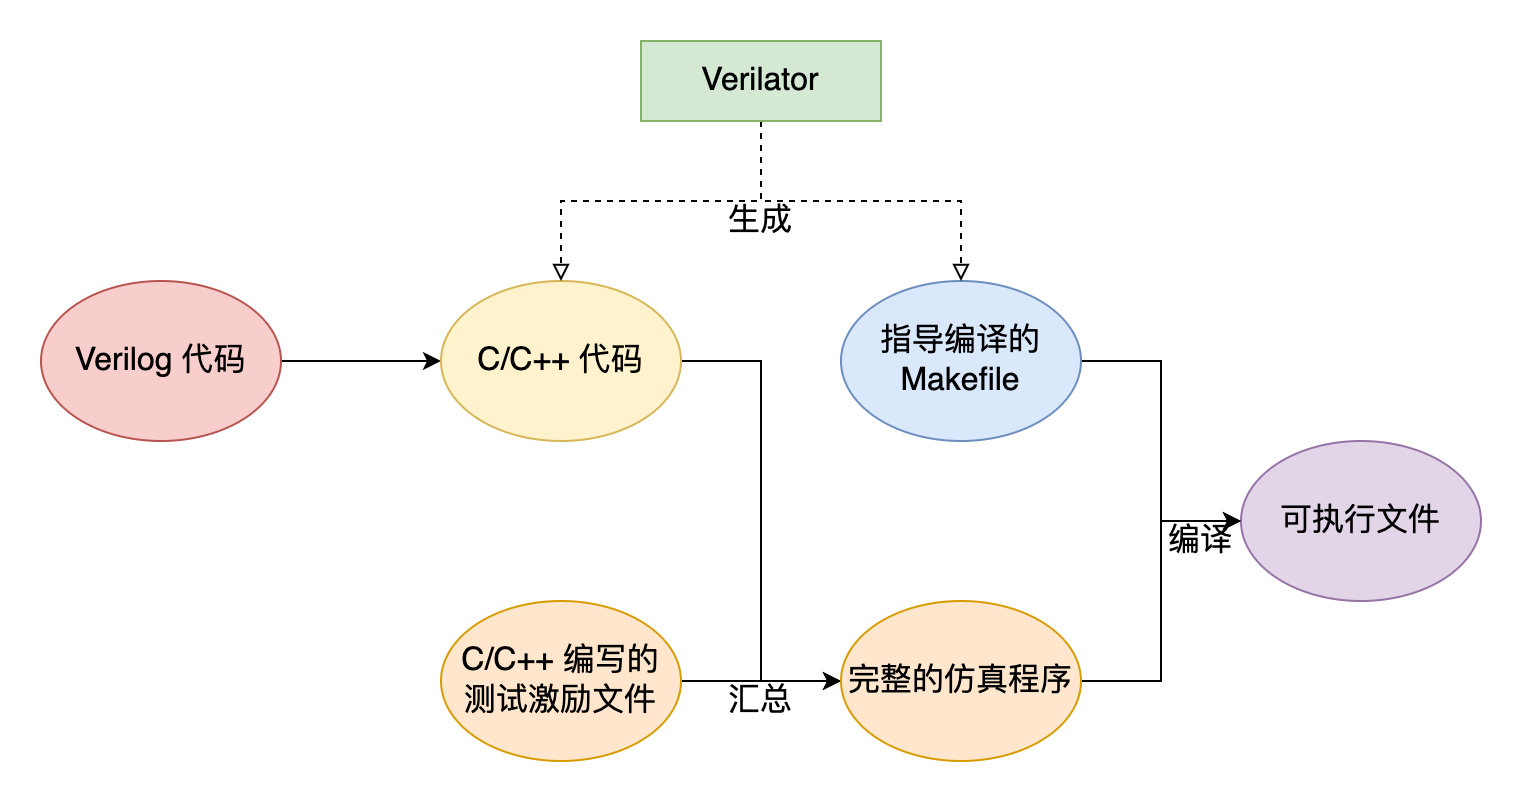
\includegraphics
          [height=.4\textheight]
          {figures/work.png}
        \end{stampbox}
        \caption{Verilator 工作原理}
      \end{figure}
    \end{column}
    \textcolor{cprimary}{\vrule}\hfill
    \begin{column}{.5\textwidth}
      \alert{\textbf{Verilator 工作流程}}
      \stamphrule
      \begin{enumerate}
        \item 硬件设计转化为一个处理器模拟器的软件。
        \item 使用 C/C++ 编写激励文件。
        \item 利用 GCC 等编译器将生成的 C/C++ 文件和我们编写的激励文件编译成成用于仿真的可执行文件。
      \end{enumerate}
    \end{column}
  \end{columns}
  \note[item]{首先,Verilator 将 Verilog 代码中并行的各个逻辑部件以合适的顺序串行化,使硬件设计转化为一个类似于处理器模拟器的软件;}
  \note[item]{接着,我们需要使用 C/C++ 编写激励文件。Verilator 为我们提供了顶层模块输入/输出引脚的接口,使我们得以对顶层模块的输入信号赋值或读取其输出信号。与使用 Vivado 仿真不同的是,我们可以实时地输出一些调试信息;要查看波形图时,需要将波形图导出到文件;}
  \note[item]{最后,Verilator 会生成一个 Makefile 脚本,利用 GCC 等编译器将生成的 C/C++ 文件和我们编写的激励文件编译成成用于仿真的可执行文件。}
\end{frame}

\begin{frame}[fragile]
  \frametitle{Verilator 激励代码}
  节选自 \href{https://github.com/verilator/verilator/blob/a187a16e56e9d4f4435bcdc62fdf77f0600cd2d7/examples/make_hello_c/sim_main.cpp\#L14}{Verilator 官方激励代码示例}。
  \begin{codeblock}[language=c++]{节选}
VerilatedContext* const contextp = new VerilatedContext;
contextp->commandArgs(argc, argv);
Vtop* const top = new Vtop{contextp};
while (!contextp->gotFinish()) {
    top->eval();
  }
top->final();
  \end{codeblock}
  \note[item]{构造一个 VerilatedContext 来保存模拟时间等。}
  \note[item]{传递参数,以便经过验证的代码可以看到它们,在创建任何模型之前需要调用它.}
  \note[item]{根据 Verilating "top.v" 生成的 Vtop.h 构建 Verilated 模型}
  \note[item]{模拟直到finish}
  \note[item]{评估模型}
  \note[item]{最终模型清理}
\end{frame}

\section{Scala 简介}

\subsection{Scala 语言简介}

\begin{frame}
  \frametitle{Scala 语言}
  \begin{enumerate}
    \item \paragraph{目的} \href{https://www.scala-lang.org/}{Scala} 是一门多范式的编程语言,设计初衷是要集成面向对象编程和函数式编程的各种特性。
    \item \paragraph{编译} Scala 运行于 Java 平台(Java 虚拟机),并兼容现有的 Java 程序。
    \item \paragraph{特性} Scala是一种纯面向对象的语言、函数式语言、强静态类型语言。
  \end{enumerate}
  \begin{alertblock}{语言提示}
    \emph{scale} 一词指\emph{规模、尺度、比例},而 \emph{scala} 没有意思。请在搜索时注意拼写。
  \end{alertblock}
\end{frame}

\begin{frame}[fragile]
  \frametitle{Scala 代码示例}
  \begin{codeblock}[language=scala]{Hullo World!}
object HelloWorld extends App {
    println("Hello, world!")
  }
  \end{codeblock}
\end{frame}

\subsection{Scala 实践}

\begin{frame}
  \frametitle{Scale 安装}
  \label{scalainstall}
  参考 \href{https://www.chisel-lang.org/docs/installation}{Installation}。
  \begin{itemize}
    \item Java Development Kit: 安装 \lstinline|openjdk-21-jdk| 包。
    \item \href{https://www.scala-sbt.org/}{SBT}: 安装 \lstinline|sbt| 包。
  \end{itemize}
\end{frame}

\begin{frame}[fragile]
  \frametitle{Scala 编译}
  将代码示例存入 \verb|HelloWorld.scala|。运行下列命令编译。
  \begin{codeblock}[language=bash]{编译 Scala 源代码}
scalac HelloWorld.scala  // 把源码编译为字节码
scala HelloWorld  // 把字节码放到虚拟机中解释运行
      \end{codeblock}
\end{frame}

\subsection{ScalaTest}

\begin{frame}
  \frametitle{ScaleTest 简介}
  \href{https://www.scalatest.org/}{ScalaTest} 是 Scala 生态系统中最灵活、最受欢迎的测试工具。
  
  与构建它的 Scala 语言一样,ScalaTest 旨在随着用户的需求而增长:您可以轻松扩展和组合 ScalaTest 的核心组件,以满足您可能有的任何特殊需求。因此,ScalaTest 可以扩展到各种规模的项目,从探索新想法的个人到协作开发关键任务软件的大型团队。

  ScalaTest 缩小规模的一种方式是,尽管ScalaTest 具有丰富的功能集,但它很容易上手。基于您从其他测试框架的经验中获得的知识,您可以通过 ScalaTest快速提高工作效率。
  %https://blog.csdn.net/weixin_43681766/article/details/125583958
\end{frame}


\begin{frame}[fragile]
  \frametitle{ScaleTest 代码示例}
  在包含了 \lstinline|"org.scalatest" %% "scalatest" % "3.2.18" % "test"| 库后,可以使用下列代码进行测试。
  \begin{codeblock}[language=scala]{Hullo ScalaTest!}
class ExampleTest extends AnyFlatSpec with Matchers {
    "Integers" should "add" in {
        val i = 2
        val j = 3
        i + j should be (5)
    }
}
  \end{codeblock}
  %https://blog.csdn.net/weixin_43681766/article/details/125583958
\end{frame}


\section{Chisel 简介}

\subsection{Chisel 库简介}

\begin{frame}
  \frametitle{Chisel 简介}
  \begin{enumerate}
    \item \paragraph{用途} \href{https://github.com/chipsalliance/chisel}{Constructing Hardware in a Scala Embedded Language (Chisel)} 是一种开源硬件描述语言,用于在寄存器传输级别描述数字电子设备和电路。
    \item \paragraph{语言} Chisel 将硬件构造添加到 Scala 编程语言中。
    \item \paragraph{目标} Chisel 可以编写复杂的、可参数化的电路生成器,从而生成可综合的 Verilog。
    \item \paragraph{手段} Chisel 可以创建可重用的组件和库,提高了设计的抽象级别,同时保留了细粒度的控制。
  \end{enumerate}
\end{frame}

\begin{frame}[fragile]
  \frametitle{Chisel 代码示例}
  以下是来自 \href{https://github.com/chipsalliance/chisel?tab=readme-ov-file#led-blink}{LED blink} 的示例。
  \begin{codeblock}[language=scala]{LED blink}
class Blinky(freq: Int, startOn: Boolean = false) extends Module {
    val io = IO(new Bundle {val led0 = Output(Bool())})
    val led = RegInit(startOn.B)
    val (_, counterWrap) = Counter(true.B, freq / 2)
    when(counterWrap) {
        led := ~led
      }
    io.led0 := led
  }
  \end{codeblock}
\end{frame}

\begin{frame}[fragile]
  \frametitle{Chisel 输出示例}
  来自 \href{https://github.com/chipsalliance/chisel?tab=readme-ov-file#led-blink}{LED blink} 的示例可以生成如下 Verilog 代码。
  \begin{codeblock}[language=verilog]{LED blink 的 Verilog 代码节选}
if (reset) begin led <= 1'h0; counterWrap_c_value <= 9'h0; end
else begin
automatic logic counterWrap = counterWrap_c_value == 9'h1F3; led <= counterWrap ^ led;
if (counterWrap) counterWrap_c_value <= 9'h0; else counterWrap_c_value <= counterWrap_c_value + 9'h1;
end
  \end{codeblock}
\end{frame}

\subsection{Chisel 实践}

\begin{frame}
  \frametitle{Chisel 安装}
  参考 \href{https://www.chisel-lang.org/docs/installation}{Installation}。
  \begin{itemize}
    \item Java Development Kit: 安装 \lstinline|openjdk-21-jdk| 包。
    \item \href{https://www.scala-sbt.org/}{SBT}: 安装 \lstinline|sbt| 包。
    \item \href{https://github.com/verilator/verilator/}{Verilator}: 安装 \lstinline|verilator| 包。
  \end{itemize}
\end{frame}

\begin{frame}
  \frametitle{Chisel 编译}
  使用 \href{https://github.com/freechipsproject/chisel-template}{Chisel Project Template} 作为模板,可以快速开始设计硬件。

  在目录中运行 \lstinline|sbt test| 可以测试当前安装是否正确。环境正常时,测试应当通过。

  在目录中运行 \lstinline|sbt run| 可以运行主程序。
\end{frame}



\begin{frame}[fragile,allowframebreaks]
  \frametitle{Chisel 基础语法}
  \begin{codeblock}[language=scala]{GCD.scala}
class ModuleSample extends Module {
  val io = IO(new Bundle {
    val a = Input(UInt(8.W))
    val b = Input(UInt(8.W))
    val minnum = Output(UInt(8.W))
    val maxnum = Output(UInt(8.W))
  })
  io.minnum := Mux(io.a <= io.b, io.a, io.b)
  io.maxnum := Mux(io.a <= io.b, io.b, io.a)
}    
  \end{codeblock}

  上述代码可以运行 \lstinline|sbt run| 生成对应的 SystemVerilog 代码。

  \begin{codeblock}[language=scala]{GCD.scala 对应 SystemVerilog 代码节选}
module ModuleSample(
  input        clock,reset,
  input  [7:0] io_a,io_b,
  output [7:0] io_minnum,io_maxnum
);
  wire _io_maxnum_T = io_a <= io_b;
  assign io_minnum = _io_maxnum_T ? io_a : io_b;
  assign io_maxnum = _io_maxnum_T ? io_b : io_a;
endmodule
\end{codeblock}
\end{frame}

\subsection{Chisel 设计验证}

\begin{frame}
  \frametitle{Chisel 设计验证}
  参见 \href{https://github.com/chipsalliance/chisel/blob/main/README.md\#design-verification}{Design Verification}。
  \begin{itemize}
    \item \href{https://github.com/chipsalliance/chisel/blob/main/svsim}{svsim} 是 Chisel 的轻量级测试库,包含在此存储库中。
    \item \href{https://github.com/ucb-bar/chiseltest}{chiseltest}(适用于 Chisel 5.0 及之前版本)是用于基于 Chisel 的 RTL 设计的包含电池的测试和形式验证库,并且是以前的 PeekPokeTester 的替代品,提供相同的基本构造,但具有简化的接口和并发支持 fork 和 join 和 Verilator 集成进行模拟。
  \end{itemize}
\end{frame}

\begin{frame}[fragile,allowframebreaks]
  \frametitle{svsim}
  \href{https://github.com/chipsalliance/chisel/blob/main/svsim}{svsim} 是 Chisel 的轻量级测试库,包含在 Chisel 中。它是一个用于编译和控制 SystemVerilog 模拟的低级库,目前以 Verilator 和 VCS 作为后端。
  \par
  Chisel 中可以使用 expect 来进行断言。通过对输入进行操作,然后让时钟前进一个周期即可获取结果。
      \begin{codeblock}[language=scala]{GCDSpec.scala}
class GCDSpec extends AnyFreeSpec with Matchers {
  "min and max check" in {
    simulate(new ModuleSample) { dut =>
      var a,b : Int =100;
      dut.io.a.poke(a);dut.io.b.poke(b);dut.clock.step()
      dut.io.minnum.expect(min(a,b),"Min Value test failed.");dut.io.maxnum.expect(max(a,b),"Max Value test failed.")
    }
  }
}    
          \end{codeblock}

\newpage

Chisel 中可以使用 println 输出任何东西。
\begin{codeblock}[language=scala]{GCDSpec.scala}
class GCDSpec extends AnyFreeSpec with Matchers {
  "min and max check" in {
    simulate(new ModuleSample) { dut =>
      var a,b : Int =100;
      dut.io.a.poke(a);dut.io.b.poke(b);dut.clock.step()
      println("Result: " +a.toString+" & "+b.toString+" = "+dut.io.minnum.peek().toString)
    }
  }
}    
    \end{codeblock}
  \end{frame}

\begin{frame}[fragile,allowframebreaks]
  \frametitle{Chiseltest}
  \begin{alertblock}{版本支持}
    \href{https://github.com/chipsalliance/chisel/releases/tag/v6.0.0}{Chisel 6.0.0} 在 2024 年 1 月 19 日发布。根据 \href{https://www.chisel-lang.org/docs/appendix/versioning}{Chisel Project Versioning} 的约定,主要版本更新不会提供向前的兼容性。而根据 \href{https://github.com/ucb-bar/chiseltest/issues/699}{ucb-bar/chiseltest\#699},该库尚未对 \href{https://github.com/chipsalliance/chisel/releases/tag/v6.0.0}{Chisel 6.0.0} 提供支持。下列内容未经验证,仅供参考。
    \end{alertblock}

    \href{https://github.com/ucb-bar/chiseltest/}{Chiseltest} 是用于基于 Chisel 的 RTL 设计的包含电池的测试和形式验证库。 Chiseltest 强调测试的轻量级(最小化样板代码)、易于读写(可理解性)和组合(为了更好的测试代码重用)。同时,它提供更加复杂的多线程测试等。

    以下代码为队列测试的示例,见\href{https://github.com/ucb-bar/chiseltest/blob/0783f2789981c340e7486578c6210ed8b97c4ec2/src/test/scala/chiseltest/tests/QueueTest.scala\#L48C3-L59C4}{QueueTest.scala}。

    \begin{codeblock}[language=scala]{GCDSpec.scala}
it should "work with a combinational queue" in {
  test(new PassthroughQueue(UInt(8.W))) { c =>
    c.in.initSource();c.out.initSink()
    fork {
      c.in.enqueueSeq(Seq(42.U, 43.U, 44.U))
    }.fork {
      c.out.expectDequeueSeq(Seq(42.U, 43.U, 44.U))
    }.join()
  }
} 
  \end{codeblock}
\end{frame}

% \begin{frame}
%   \frametitle{Chisel 其他}
%   TODO%https://blog.csdn.net/weixin_43681766/article/details/125582801
% \end{frame}

\subsection{Chisel 和 VS Code}

\begin{frame}
  \frametitle{VS Code 对 Chisel 的支持}
  Chisel 是一个 Scala 库。因此 Chisel 主要使用 Scala 的相关插件。为支持 Chisel 的,VS Code 主要使用 3 个插件。
  \begin{itemize}
    \item \href{https://marketplace.visualstudio.com/items?itemName=scalameta.metals}{scalameta.metals}: Scala 感知和 sbt 相关支持。
    \item \href{https://marketplace.visualstudio.com/items?itemName=scala-lang.scala}{scala-lang.scala}: Scala 语法高亮
    \item \href{https://marketplace.visualstudio.com/items?itemName=aaronduino.chisel}{aaronduino.chisel}: Chisel 语法和代码块支持。
  \end{itemize}
\end{frame}

\begin{frame}
  \frametitle{VS Code 的 Chisel 效果}
  \begin{figure}
    \centering
    \begin{stampbox}
      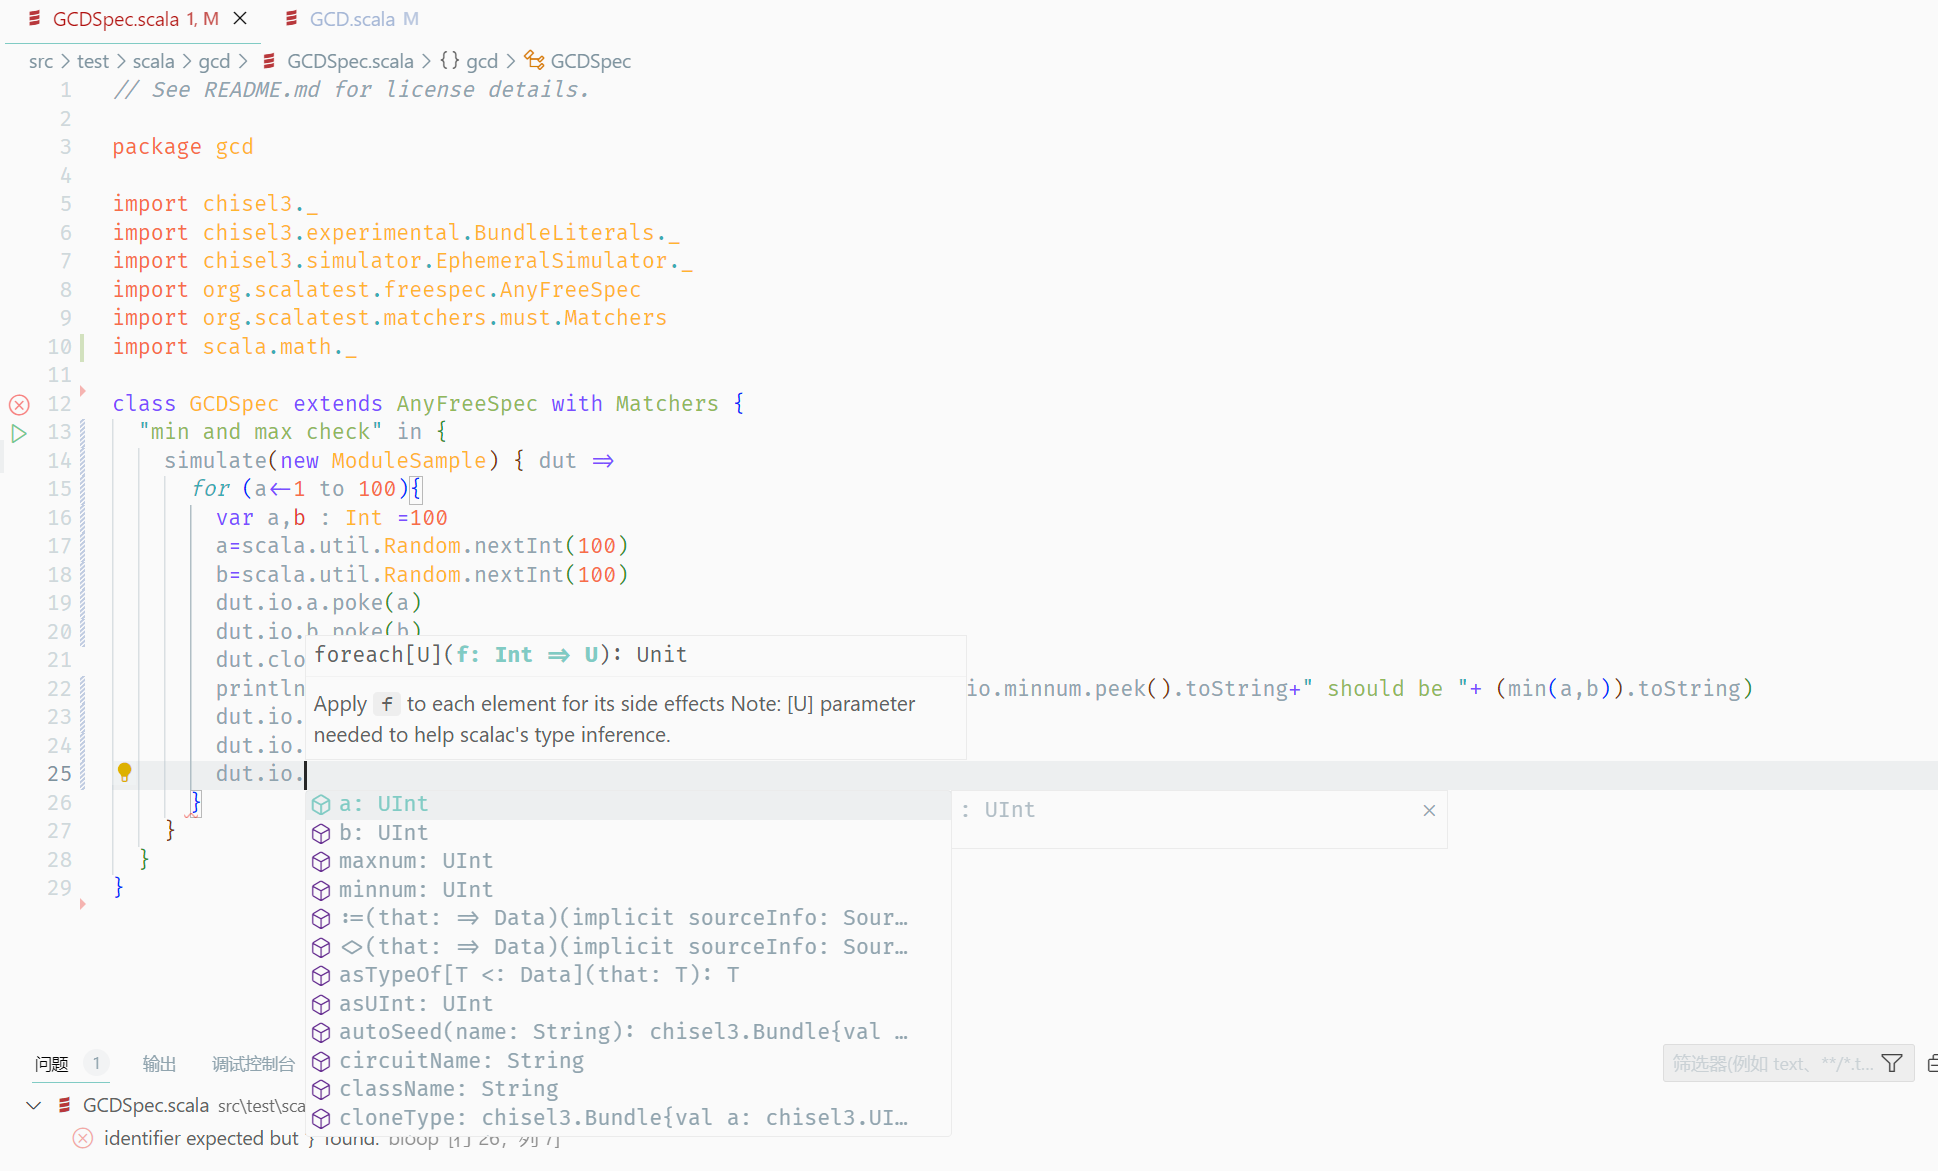
\includegraphics
      [height=.5\textheight]
      {figures/vsc.png}
    \end{stampbox}
    \caption{VS Code 的 Chisel 智能感知和静态检查演示}
  \end{figure}
\end{frame}

\subsection{测试 Chisel}

\begin{frame}[fragile,allowframebreaks]
  \frametitle{测试 Chisel}
  参考 \href{https://www.chisel-lang.org/docs/installation}{Installation},首先安装所需的依赖项才能在本地构建 Chisel,安装 \lstinline|openjdk-21-jdk| 包、安装 \lstinline|sbt| 包、安装 \lstinline|verilator| 包。

  运行下列代码克隆并构建 Chisel。

  \begin{codeblock}[language=bash]{构建 Chisel}
git clone https://github.com/chipsalliance/chisel.git
cd chisel
sbt compile
  \end{codeblock}

  为了运行单元测试,PATH 中应包含 \href{https://www.veripool.org/verilator/}{verilator}、\href{https://yosyshq.net/yosys/}{yosys} 和 \href{https://github.com/chipsalliance/espresso}{espresso}。

  \newpage

  如果编译成功并且安装了上述依赖项,则可以通过调用以下命令来运行包含的单元测试。

  \begin{codeblock}[language=bash]{构建 Chisel}
sbt test
  \end{codeblock}
\end{frame}

\section{Chisel 和 RISC-V}

\subsection{在 openEuler RISC-V 上运行 Chisel}

% \subsubsection{Chisel 依赖在各 RISC-V 发行版上的情况对比}

% \begin{frame}
%   \frametitle{对比}
%   TODO%https://blog.csdn.net/weixin_43681766/article/details/125582801
% \end{frame}

\subsubsection{在 openEuler RISC-V 上运行 Chisel}

% \begin{frame}
%   \frametitle{运行}
%   TODO%https://blog.csdn.net/weixin_43681766/article/details/125582801
% \end{frame}

\begin{frame}[fragile,allowframebreaks]
  \frametitle{运行 Verilator}
  注意到 openEuler RISC-V 尚未提供 \lstinline|verilator| 包。参阅 \href{https://veripool.org/guide/latest/install.html#git-quick-install}{Git Quick Install} 的说明。

  \begin{codeblock}[language=bash]{构建 Verilator}
yum install -y git help2man perl python3 make autoconf g++ flex bison ccache numactl
git clone https://github.com/verilator/verilator --depth=1
cd verilator
autoconf
./configure
make -j `nproc`
sudo make install
  \end{codeblock}

  \newpage

  按照有关提示,运行 \lstinline|make test| 进行有关测试,部分测试可以通过,部分测试由于缺少包而无法通过或跳过测试。这说明 Verilator 能够在该系统上运行。

  \begin{codeblock}[language=bash]{Verilator 验证结果}
==SUMMARY: Passed 1  Failed 0  Time 2:55
==SUMMARY: Passed 1  Failed 0  Time 2:55
  \end{codeblock}
\end{frame}

\begin{frame}
  \frametitle{运行 Scale}
  参考 \ref{scalainstall} 安装并测试 Hullo World 程序,能够运行通过。
\end{frame}

\begin{frame}[fragile]
  \frametitle{运行 Chisel}
  参考 \href{https://github.com/freechipsproject/chisel-template?tab=readme-ov-file#did-it-work}{Did it work?} 的有关说明,在目录中运行 \lstinline|sbt -Dsbt.override.build.repos=true test --debug|,得到如下结果。猜想问题为 JVM 虚拟机内部实现可能不符合预期,需进一步排查或对 Chisel 进行进一步测试。

  \begin{codeblock}[language=bash]{构建 Verilator}
scala.MatchError: false (of class scala.reflect.internal.Trees\$Literal)
        at scala.tools.nsc.typechecker.Macros\$MacroImplBinding\$.unpickleAtom(Macros.scala:118)
        at scala.tools.nsc.typechecker.Macros\$MacroImplBinding\$\$anonfun\$7.apply(Macros.scala:186)
        at scala.tools.nsc.typechecker.Macros\$MacroImplBinding\$\$anonfun\$7.apply(Macros.scala:186)
  \end{codeblock}

  
\end{frame}

% \subsection{Chisel with RISC-V}

\subsection{使用 Chisel 的 RISC-V 项目}

\begin{frame}
  \frametitle{使用 Chisel 的 RISC-V 项目}
  \begin{itemize}
    \item \href{https://github.com/ucb-bar/riscv-sodor}{The Sodor Processor Collection}: RV32I 处理器的简易实现
    \item \href{https://github.com/OSCPU/NutShell}{NutShell}:  OSCPU(大学开源芯片项目)团队开发的处理器,目前支持 RV64IMAC 和 RV32IMAC。
    \item \href{https://github.com/freechipsproject/rocket-chip}{Rocket Chip Generator}: 一款开源片上系统设计生成器,可生成 RTL。
    \item \href{https://github.com/OpenXiangShan/XiangShan}{香山}: 一款开源的高性能 RISC-V 处理器,架构为 RV64GCBK。
    \item \href{https://github.com/ucb-bar/riscv-boom}{BOOM}: Christopher Celio 的 RV64 乱序处理器实现。
    \item \href{https://github.com/google/bottlerocket}{BottleRocket}: RV32IMC 微处理器。
  \end{itemize}
\end{frame}

% \begin{frame}
%   \frametitle{参考文献}
%   \printbibliography[heading=none]
% \end{frame}

\makebottom

\end{document}